% Ch4.tex

\chapter[Frog call classification based on enhanced features]{Frog call classification based on feature fusion and machine learning algorithms}
\label{cha:cha4EnhancedFeature}


\textbf{Research problem}
\\
Previous studies classified frog calls in high SNR recordings using one or two types of features from temporal, perceptual, and cepstral features. However, the fused feature set using one or two types of features cannot classify frog species that share similar characteristics in one or two domains (temporal domain, perceptual domain, and cepstral domain).
\\
\textbf{Research sub-question}
\\
How to build a feature set for further improving frog call classification performance in high SNR recordings?



\section{Overview}
\label{S:1}



This chapter aims to compare various feature sets using different machine learning techniques, and finds the best feature set for classifying frogs in high SNR recordings. 
Based on the classification performance, suggested features can then be adapted to study low SNR recordings. In particular, we want to know which features can be adopted from high SNR recordings to low SNR recordings, because the final goal of this thesis is to classify  multiple simultaneously vocalising frog species in low SNR recordings.

The proposed method is evaluated using twenty-four frog species, which are geographically well distributed through Queensland, Australia. Five feature sets are constructed and evaluated using five machine learning algorithms. 



\section{Methods}

Our frog call classification system contains six modules (Figure~ \ref{fig:Ch4_flowchart}): data description, syllable segmentation, pre-processing,  feature extraction, feature fusion, and classification. Detailed information of each module is described in following subsections. Different from \citep{huang2009frog}, pre-processing is directly applied to segmented syllables rather than continuous recordings.

\begin{figure}[htb!] % Example image
\center{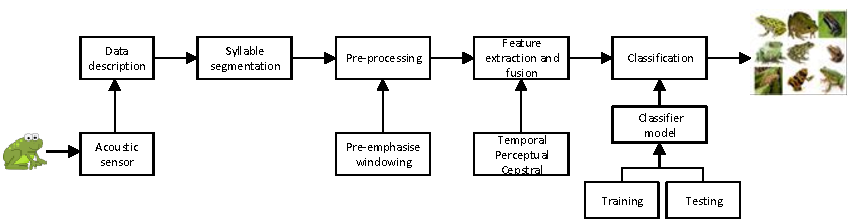
\includegraphics[width=1\linewidth]{image/Ch4/flowchart.pdf}}
\caption{Flowchart of frog call classification system using enhanced features}
\label{fig:Ch4_flowchart} 
\end{figure}


\subsection{Data description}
In this chapter, twenty-four frog species, which are widespread in Queensland, Australia, are selected for experiments (Table~\ref{tab:Ch4_frogName}). 
All those frog species are collected from commercial recordings \citep{CD}. All the recordings are two-channel, sampled at 44.10 kHz and saved in MP3 format. All recordings were obtained with a directional microphone and have a high SNR. Each recording includes one frog species with the duration ranging from eight to fifty-five seconds.

\begin{table}[htb!]
\centering
\caption[Summary of scientific name, common name, and corresponding code]{Summary of scientific name, common name, and corresponding code. Frog species name with asterisk means that it needs to be smoothed before segmentation}
\resizebox{0.7\textwidth}{!}{
\begin{tabular}{cllc}
\hline\hline
\multicolumn{1}{l}{\textbf{No.}} & \textbf{Scientific-name}      & \textbf{Common-name}   & \multicolumn{1}{l}{\textbf{Code}} \\ \hline
1                                  & \textit{Assa darlingtoni}             & Pouched frog                                                     & ADI                                \\ 
2                                  & \textit{Crinia parinsignifera}        & Eastern sign-bearing froglet                                     & CPA                                \\ 
3                                  & \textit{Crinia signifera}             & Common eastern froglet                                           & CSA                                \\ 
4                                  & \textit{Limnodynastes convexiusculus} & Marbled frog                                                    & LCS                                \\ 
5                                  & \textit{Limnodynastes ornatus}        & Ornate burrowing frog                                            & LOS                                \\ 
6                                  & \textit{Limnodynastes tasmaniensis}*   & Spotted grass frog                                              & LTS                                \\ 
7                                  & \textit{Limnodynastes terraereginae}  & Northern banjo frog                                              & LTE                                \\ 
8                                  & \textit{Litoria caerulea}             & Australian green tree frog                                      & LCA                                \\ 
9                                  & \textit{Litoria chloris}              & Red-eyed tree frog                                              & LCS                                \\ 
10                                 & \textit{Litoria latopalmata}         & Broad-palmed frog                                                & LLA                                \\ 
11                                 & \textit{Litoria nasuta}               & Striped rocket frog                                             & LNA                                \\ 
12                                 & \textit{Litoria revelata}             & Revealed tree frog                                             & LEA                                \\ 
13                                 & \textit{Litoria rubella}              & Desert tree frog                                                 & LRA                                \\ 
14                                 & \textit{Litoria tyleri}               & Southern laughing tree frog                                     & LTI                                \\ 
15                                 & \textit{Litoria verreauxii verreauxii}           & Whistling tree frog                                           & LVI                                \\ 
16                                 & \textit{Mixophyes fasciolatus}        & Great barred frog                                               & MFS                                \\ 
17                                 & \textit{Mixophyes fleayi}             & Fleay's barred Frog                                             & MFI                                \\ 
18                                 & \textit{Neobatrachus sudelli}*        & Painted burrowing frog                                           & NSI                                \\ 
19                                 & \textit{Philoria kundagungan}         & Mountain frog                                                     & PKN                                \\ 
20                                 & \textit{Philoria sphagnicolus}*        & Sphagnum frog                                                    & PSS                                \\ 
21                                 & \textit{Pseudophryne coriacea}        & Red-backed toadlet                                            & PCA                                \\ 
22                                 & \textit{Pseudophryne raveni}*          & Copper-backed brood frog                                        & PRI                                \\ 
23                                 & \textit{Uperoleia fusca}*             & Dusky toadlet                                                   & UFA                                \\ 
24                                 & \textit{Uperoleia laevigata}          & Smooth toadlet                                                 & ULA                                \\ \hline\hline
\end{tabular}
}
\label{tab:Ch4_frogName}
\end{table}



\subsection{Syllable segmentation based on an adaptive end point detection}
\label{Ch3:segmentationProcess}

Each recording is made up of multiple continuous calls of one frog species. For frogs, one syllable is an elementary acoustic unit for classification, which is a continuous vocalisation emitted from an individual \citep{huang2009frog}. In this chapter, one method built on the H$\ddot{a}$rm$\ddot{a}$'s method is used to perform syllable segmentation for frog calls \citep{harma2003automatic}. The syllable segmentation process is based on the spectrogram, which is generated by applying STFT to each recording. For STFT, the window function used is Hamming window with the size and overlap being 512 samples and 25\%, respectively. The detail of the segmentation method is described in Figure~\ref{fig:segmentation}, which is based on the iterative frequency-amplitude information of the spectrogram. This chapter focuses on the evaluation of fused features, but the accuracy of segmentation results can greatly affect the classification performance. To reduce the bias introduced by syllable segmentation, the segmented syllables are further filtered. First, those syllables whose length are smaller than 300 samples are removed. Then, those syllables whose averaged energy is smaller than 15\% of the maximum energy and larger than 1.5 times the averaged energy are removed for each frog species experimentally \citep{Gingras2013}.


\begin{figure}[htb!] % Example image
\center{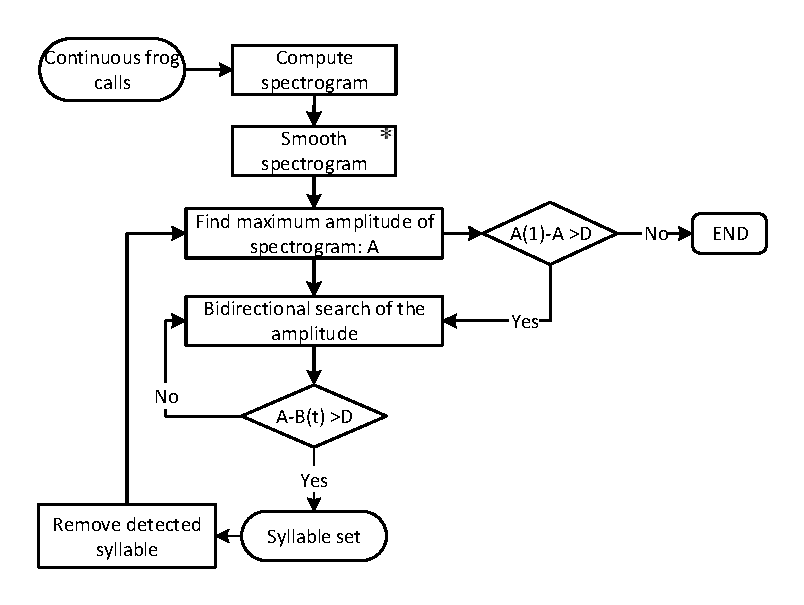
\includegraphics[width=0.8\linewidth]{image/Ch4/segmentation.pdf}}
\caption[H$\ddot{a}$rm$\ddot{a}$'s segmentation algorithm]{Segmentation method based on H$\ddot{a}$rm$\ddot{a}$'s algorithm. Here, $D$ is the amplitude threshold for stopping criteria which is set at 20 dB experimentally, and the segmentation result is sensitive with this value. $A$ is the maximum amplitude value of the spectrogram and we save the first maximum amplitude as $A(1)$, $B(t)$ is the amplitude of frame $t$. An asterisk denotes the optional processing step.}
\label{fig:segmentation} 
\end{figure}



In this chapter, smoothing spectrogram is optionally applied to the spectrogram before the H$\ddot{a}$rm$\ddot{a}$'s algorithm, because some frog species have a large temporal gap within one syllable (see in Figure~\ref{fig:smooth}). As for the smoothing, a Gaussian filter (7$\times$7) is applied to the spectrogram, where the size is set, taking into account a trade-off between connecting gaps within one syllable and separating adjacent syllables. The segmentation result after smoothing is shown in Figure~\ref{fig:smooth}. The distribution of syllable numbers after segmentation for all frog species is shown in Figure~\ref{fig:Ch4_syllable}.

\begin{figure}[htb!]
\centering
        \begin{subfigure}[b]{0.6\linewidth}
                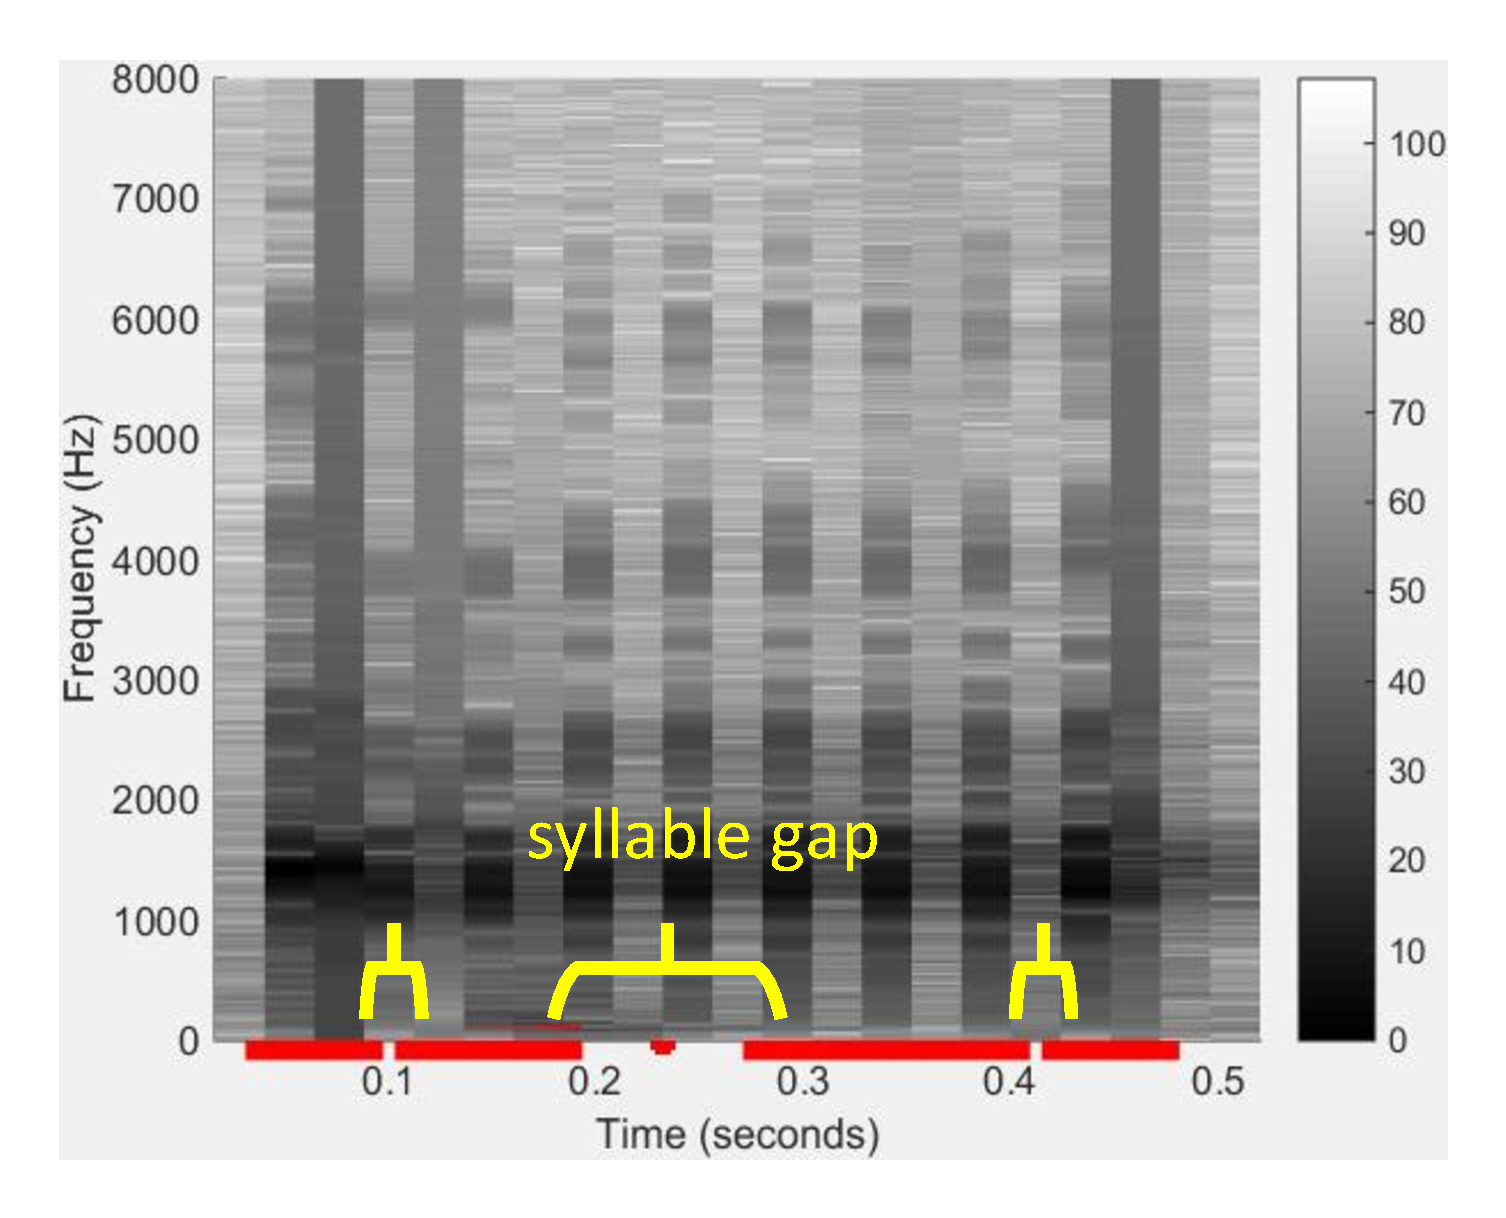
\includegraphics[width=\textwidth]{image/Ch4/no.pdf}
                \caption{Before smoothing}
        \end{subfigure}%
        \\ 
        \begin{subfigure}[b]{0.6\linewidth}
                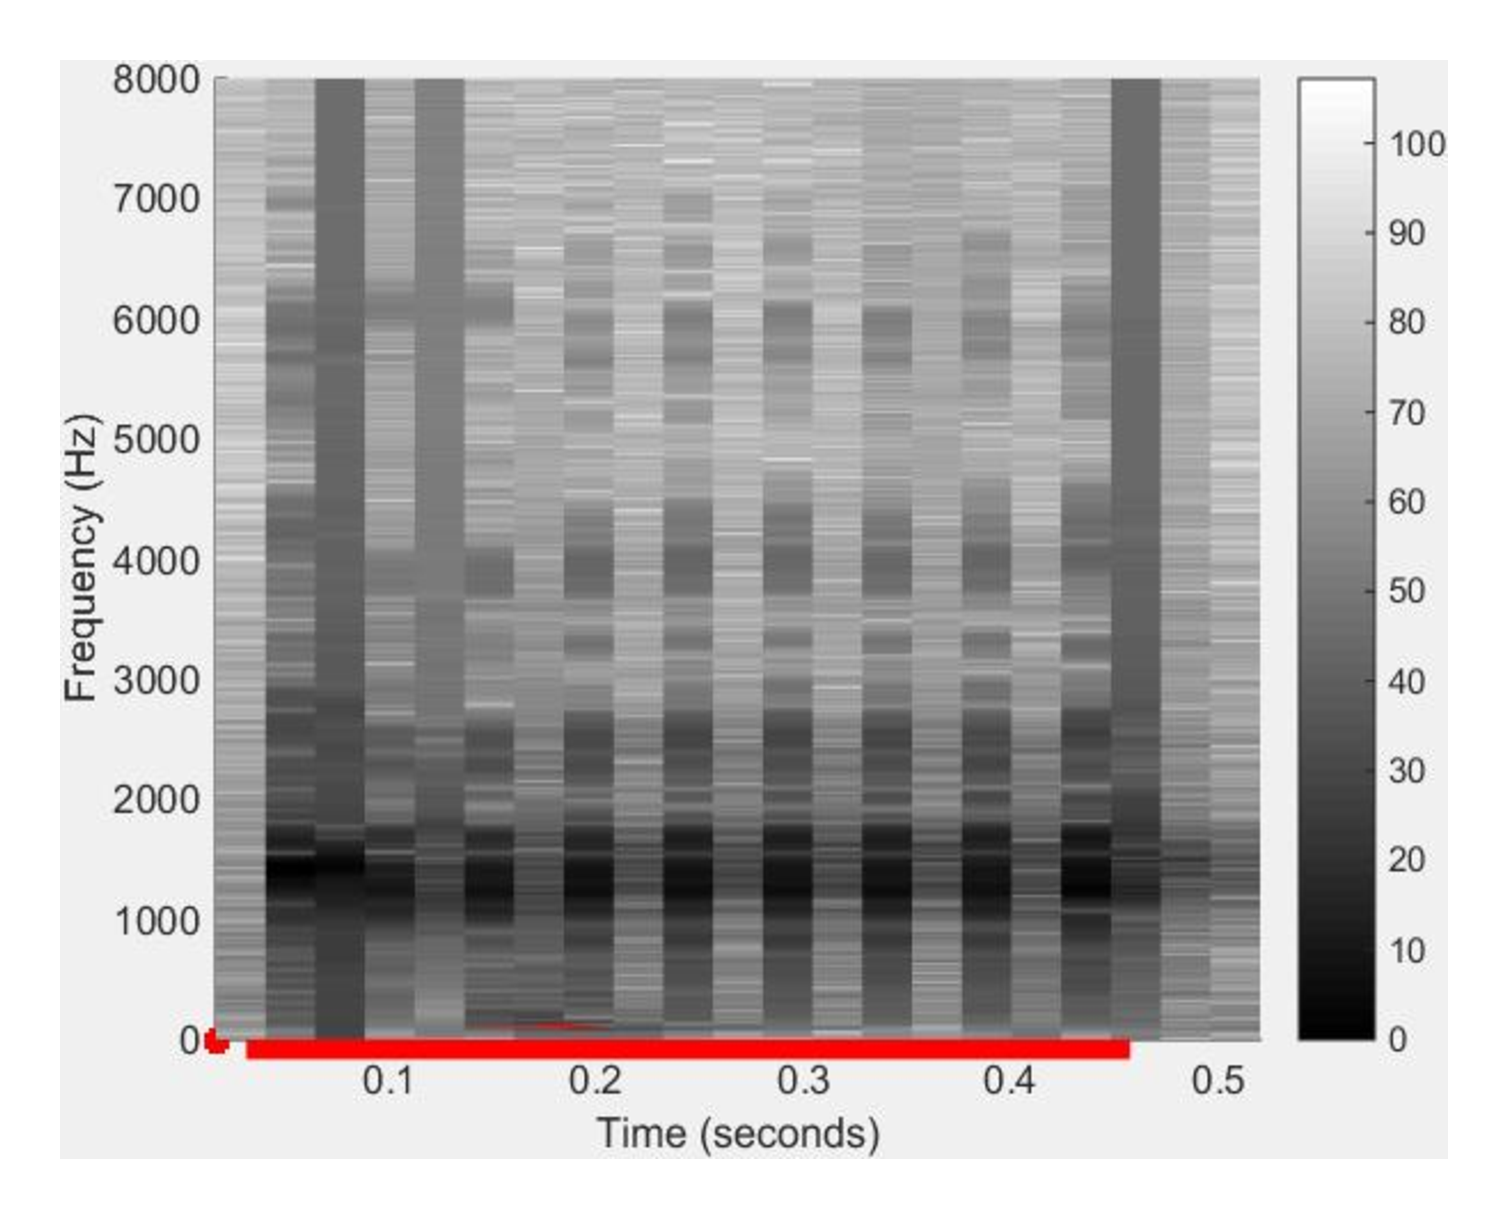
\includegraphics[width=\textwidth]{image/Ch4/yes.pdf}
                \caption{After smoothing}
        \end{subfigure}
        \caption[Syllable segmentation results]{Syllable segmentation results are marked with a red
line for \textit{Neobatrachus sudelli} (one syllable).}       
        \label{fig:smooth}
\end{figure}



\begin{figure}[htb!] % Example image
\center{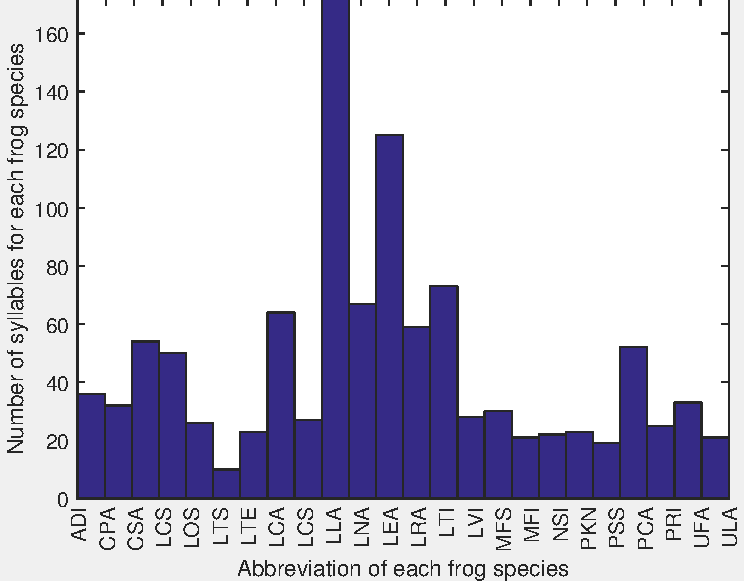
\includegraphics[width=0.6\linewidth]{image/Ch4/syllable.pdf}}
\caption[Distribution of syllable number for all frog species]{Distribution of syllable number for all frog species. The x-axis is the abbreviation of each frog species, and the corresponding scientific name can be found in Table \ref{tab:Ch4_frogName}.}
\label{fig:Ch4_syllable} 
\end{figure}


\subsection{Pre-processing}
Since features play an important role in the classification performance, pre-processing is applied to each syllable to improve the accuracy of feature extraction. The pre-processing of each syllable consists of the following steps:

\subsubsection{Pre-emphasise}
Some collected frog calls have low amplitude but in the high frequency, which will have an effect on feature extraction of the spectrum at the high frequency end. To enhance those high-frequency components and reduce the low-frequency components, a first-order high-pass filter with finite impulse response is introduced and defined as

\begin{align}
y(n) = s(n)-\alpha s(n-1)
\end{align}

where $s$ denotes a frog syllable, $y$ is the output of the high-pass filter, $\alpha$ denotes the cut-off frequency of the high-pass filter and is set at 0.97 here, $n$ is the n-th sample of the syllable. 

\subsubsection{Windowing}
After pre-emphasis, each syllable is segmented into overlapping frames with fixed length. A Hamming widow is used to minimise the maximum side-lobe in the frequency domain and get side-lobe suppression, which is defined as

\begin{equation}
w(n)=0.54-0.46cos(\frac{2n\pi}{L-1}), 0 \leq n \leq L-1
\end{equation}
where $L$ is the length of the frame. Because window sizes have an effect on the classification results, different window sizes are optimised for different features in this chapter. The signal after windowing process is expressed as
\begin{equation}
x(n) = w(n)y(n)
\end{equation}

\subsection{Feature extraction}
After pre-processing of each syllable, various parametric representations are used to represent the syllable. In the literature, a variety of parametric representations of frog calls can be found, such as LPCs and MFCCs \citep{yuan2013frog, jaafar2013automatic, bedoya2014automatic}.
MFCCs achieved better performance than LPCs \citep{yuan2013frog}. Different from the hybrid features used \citep{huang2009frog, han2011acoustic, Gingras2013}, our enhanced  feature consists of more features, such as oscillation rate \citep{Xie1504:Acoustic}, to further improve the classification accuracy. In this chapter, temporal features include syllable duration, Shannon entropy, r$\acute{e}$nyi entropy, zero-crossing rate, averaged energy, and oscillation rate. Perceptual features contains spectral centroid, spectral flatness, spectral roll-off, signal bandwidth, spectral flux, and fundamental frequency. Here the word \textit{perceptual} is defined according to \citep{lei2014content}. MFCCs are used as a cepstral feature. The description of each feature is listed below.

\vspace{3mm}

\noindent(1) Syllable duration: Syllable duration \citep{Xie1504:Acoustic} is directly obtained from the bounds (time domain) of the segmentation results.
\begin{equation}
Dr = x(n_{e}) - x(n_{s})
\end{equation}
where $n_{e}$ and $n_{s}$ are the end and start location of one segmented syllable.

\vspace{3mm}

\noindent(2) Shannon entropy: Shannon entropy is the expected information content of a sequence of a signal. It is often used to describe the average of all the information contents weighted by their probabilities $p_{i}$.
\begin{equation}
Se=-\sum_{i=1}^{L}p_{i}log_{2}(p_{i})
\end{equation}
where $L$ is the length of a frog syllable.

\vspace{3mm}

\noindent(3) R$\acute{e}$nyi entropy: r$\acute{e}$nyi entropy is calculated to obtain the different averaging of probabilities via the parameter $\alpha$, and defined as

\begin{equation}
Re=\frac{1}{1-\alpha}log_{2}(\sum_{i}^{n}p_{i}^{\alpha})
\end{equation}
where $p_{i}$ is the probabilities of the occurence x(n) in the signal.

\vspace{3mm}

\noindent(3) Zero-crossing rate: zero-crossing rate denotes the rate of signal change along a signal. When adjacent signals have different signs, a zero-crossing occurs. The mathematical expression of $ZCR$ can be defined as
\begin{equation}
Zcr=\frac{1}{2}\sum_{n=0}^{L-1}[sgn(x(n))-sgn(x(n+1))]
\end{equation}

\vspace{3mm}

\noindent(4) Averaged energy: Averaged energy is defined as the sum of intensity of signal.
\begin{equation}
Ae = \frac{1}{L}\sum_{n=0}^{L-1}x(n)^{2}
\end{equation}


\vspace{3mm}
\noindent(5) Oscillation rate: Oscillation rate is calculated in the frequency boundary around the fundamental frequency. First, the power within the frequency boundary is calculated. After normalising the power, the first and last 20\% part of the power vector is discarded due to the uncertainty. Next, the autocorrelation is performed by the length of the vector. Furthermore, a discrete cosine transform is employed to the vector after mean subtraction, and the position of the highest frequency is achieved to calculate the oscillation rate. 

%Detailed description can be found in our previous study \citep{Xie1504:Acoustic}.




\vspace{3mm}
\noindent(6) Spectral centroid: spectral centroid is the centre point of spectrum distribution. In terms of human audio perception, it is often associated with the brightness of the sound. With the magnitudes as the weight, it is calculated as the weighted mean of the frequencies.
\begin{equation}
Sc=\frac{\sum_{k=0}^{N-1}f_{k}X(k)}{\sum_{k=0}^{N-1}X(k)}
\end{equation}
where $X(k)$ is the discrete Fourier transform (DFT) of the syllable signal of the k-th frame, N is the half size of DFT. 

\vspace{3mm}
\noindent(7) Spectral flatness: spectral flatness provides a way to quantify the tonality of a sound. A higher spectral flatness indicates a similar amount of power of the spectrum in all spectral bands. Spectral flatness is measured by the ratio between the geometric mean and the arithmetic mean of the power spectrum and defined as
\begin{equation}
Sf = \frac{exp(\frac{1}{N}\sum_{k=0}^{N-1}InX(k))}{\frac{1}{N}\sum_{k=0}^{N-1}X(k)}
\end{equation}

\vspace{3mm}

\noindent(8) Spectral roll-off: spectral roll-off is often used to measure the spectral shape, and defined as the frequency $H$. Here $H$ is the value below which the $\theta$ of the magnitude distribution is concentrated.

\begin{equation}
\sum_{k}^{H}X(k)=\theta \sum_{k=1}^{N-1}X(k)
\end{equation}
where $\theta$ is set at 0.85.

\vspace{3mm}

\noindent(9) Signal bandwidth: signal bandwidth can be used to represent the difference between the upper and lower cut-off frequencies.

\begin{equation}
Bw=\sqrt{\frac{\sum_{k=0}^{N-1}(k-Sc)^{2}|x(n)|}{\sum_{k=0}^{N-1}X(k)}}
\end{equation} 

\vspace{3mm}

\noindent(10) Spectral flux: spectral flux is used to measure how quickly the power spectrum of a signal is changing. The spectral flux can be obtained via the power spectrum comparison between one frame and its previous one. The calculation of spectral flux is denoted as
\begin{equation}
Sf = \sum_{k=-\frac{N}{2}}^{k=\frac{N}{2}}H[|X(n,k)|-|X(n-1,k)|]
\end{equation}
where $H(x)=(x+|x|)/2$ is a half-wave rectifier function.

\vspace{3mm}

\noindent(11) Fundamental frequency: fundamental frequency is calculated via averaging peak intensity of all frames within one frog syllable. If the peak intensity value is higher than an empirically chosen or specified threshold, the frequency of that peak will be selected to calculate the fundamental frequency.

\vspace{3mm}

\noindent(12) Mel-frequency cepstral coefficients (MFCCs): MFCCs, which are obtained by applying cosine transform to a sub-band Mel-frequency spectrum within a short time, have been widely used in bird classification \citep{lee2006automatic}, speech/speaker recognition \citep{han2006efficient}, and frog identification \citep{bedoya2014automatic}. In this chapter, MFCCs are calculated based on the method of \citep{lee2006automatic}. 

\noindent  \textbf{Step 1}: Band-pass filtering: The amplitude spectrum is then filtered using a set of triangular band-pass filters.
\begin{equation}
E_{j}=\sum_{k=0}^{N/2-1}\phi_{j}(k)A_{k}, 0 \leq j \leq J-1
\end{equation}
where J is the number of filters, $\phi_{j}$ is the $j^{th}$ filter, and $A_{k}$ is the amplitude of $X(k)$.
\begin{equation}
A_{k}=|X[k]|^{2}, 0 \leq k \leq N/2
\end{equation}
\noindent  \textbf{Step 2}: Discrete cosine transform: MFCCs for the $i^{th}$ frame are computed by performing DCT on the logarithm of $E_{j}$. 
\begin{equation}
C_{m}^{j} = \sum_{j=0}^{J-1}\cos(m \frac{\pi}{J}(j+0.5))log_{10}(E_{j}), 0 \leq m \leq L-1
\end{equation}
where $L$ is the number of MFCCs.

In this chapter, the filter bank consists of 40 triangular filters, that is  $J=40$. The length of MFCCs of each frame is 12 (L=12). After calculating MFCCs from each frame, the averaged MFCCs of all frames within one syllable are calculated as
\begin{equation}
f_{m}= \frac{\sum_{i=1}^{K}(C_{m}^{l})}{K}, 0\leq m \leq L-1
\end{equation}
where $f_{m}$ is the $m^{th}$ MFCCs, $K$ is the number of frames within the syllable. 

For all perceptual features and $Zcr$, the mean values are calculated to characterise the frog syllable. Then, the L-dimensional MFCC vectors are fused with the other 11 feature vectors to form the enhanced temporal, perceptual and cepstral (TemPerCep) features.

After the formulation of feature vectors, normalisation is conducted as 
\begin{equation}
v_{i} = \frac{v_{i}-\mu_{i}}{\sigma_{i}}
\end{equation} 
where $\mu_{i}$ and $\sigma_{i}$ are the mean and standard deviation computed for each feature vector $i$.  

Let $F_{1}$ represent temporal features with length $L_{1}$, $F_{2}$ and $F_{3}$ represent perceptual features and cepstral features with length $L_{2}$ and $L_{3}$, respectively. The enhanced procedure is performed as
\begin{equation}
F_{H} = w_{1}F_{1}\oplus w_{2}F_{2} \oplus w_{3}F_{3}
\end{equation} 
where $w_{1}$, $w_{2}$, and $w_{3}$ are the weights, $\oplus$ is the concatenation operation.


\subsection{Classifier description}

\label{ch4:classifierDesign}
In this chapter we report the results for five classification algorithms: 1) LDA, 2) kNN, 3) SVM, 4) RF, 5) ANN. Five feature vectors, LPCs, MFCCs, fused temporal feature and MFCCs (\textit{TemCep}), fused temporal and perceptual features (\textit{TemPer}), fused temporal, perceptual features, and MFCCs (\textit{TemCepPer}), are fed into each classifier respectively to test their classification performance.

\subsubsection{Linear discriminant analysis}
After transforming the feature vector into low-dimensional space, the classification accuracy can be improved for LDA. In LDA, the goal is to find an optimal transformation matrix to transform the feature vector from an n-dimensional space to a d-dimensional space. A linear mapping, which maximises the Fisher criterion $J_{F}$, is used to obtain the transformation matrix as
\begin{equation}
J_{F}(A)=tr((A^{T}S_{w}A)^{-1}(A^{T}S_{B}A))
\end{equation}
where $S_{w}$ and $S_{B}$ are the within-class scatter matrix and between-class scatter matrix, respectively. The within-class scatter matrix and between-class scatter matrix are respectively defined as 

\begin{equation}
S_{W}=\sum_{j=1}^{C}\sum_{i=1}^{N_{j}}(F_{i}^{j}-\mu_{j})(F_{i}^{j}-\mu_{j})^{T}
\end{equation}

\begin{equation}
S_{B}=\sum_{j=1}^{C}(\mu_{i}-\mu)(\mu_{i}-\mu)^{T}
\end{equation}
where $F_{i}^{j}$ is the i-th feature vector of frog species $j$, $\mu_{j}$ is the mean vector of species $j$, $C$ is the number of frog species, and $N_{j}$ is the number of feature vectors in species $j$, $\mu$ is the mean vector of all frog species.

The optimisation of the transform matrix can be determined via finding the eigenvectors of $S_{W}^{-1}S_{B}$.

\begin{equation}
A_{opt}= argmax \frac{tr(A^{T}S_{B}A)}{A^{T}S_{W}A}
\end{equation}

In the recognition stage, the feature vector is first transformed into a lower-dimensional space via $A_{opt}$ derived by LDA. Then, the distance between the feature vector of the test syllable and the feature vector representing this species is calculated. The one with minimum distance is regarded as the identified species.

\subsubsection{K-nearest neighbour}
For the kNN classifier, an object is classified to the majority class of its $k$ nearest neighbours \citep{huang2009frog}. Specifically, in the training phase, frog feature vectors are stored with species labels. For the test phase, the simplest classification combination method is the voting method. The $k$ closet vectors are selected for voting, then the classification for the input feature vector $f_{i,c}$ is assigned with the majority class.

The second classification combination method is to calculate the average distance between an input frog feature vector and $k$ closest vectors. For example, the Euclidean distance between an input feature vector $f_{i,c}$ and one stored feature vector $f_{j,c}$ is calculated as
\begin{equation}
d(i,j) = \sqrt{\sum_{c=1}^{n}(f_{i,c}-f_{j,c})^2}
\end{equation}
\noindent where $i$ and $j$ are indices of the feature vector, $n$ means the dimension of the feature vector. Next, \textit{k} nearest neighbours of feature vector $i$ are selected based on the Euclidean distance for voting. If the following equation is satisfied
\begin{equation}
\frac{1}{k_{1}}\sum_{j \in s_{1}} d(i,j(s_{1})) < \frac{1}{k_{2}}\sum_{j \in s_{2}}d(i,j(s_{2})) 
\end{equation}
\noindent where $k=k_{1}+k_{2}$, $k_{1}$ is the number of frog species $s_{1}$, $k_{2}$ is the number of frog species $s_{2}$. Here, the input feature vector $i$ will be classified as frog species $s_{2}$.

The third classification combination method is to calculate the sum of similarity of $k$ closest feature vectors. For a binary classification task with two classes: $k_{1}$ and $k_{2}$. If

\begin{equation}
\sum_{j \in s_{1}} d(i,j(s_{1})) < \sum_{j \in s_{2}}d(i,j(s_{2}))
\end{equation}
Then the input feature vector $i$ will be classified as belonging to class $s_{2}$. Following prior work (\citep{han2011acoustic, Xie1504:Acoustic}), the distance function used for kNN is the Euclidean function, and $k$ is set at 1.

\subsubsection{Support vector machines}
Due to the high accuracy and superior generalisation properties, SVM has been widely used for classifying animal sounds \citep{huang2009frog} \citep{acevedo2009automated}. In this chapter, the feature set obtained is first selected as training data. Then, the pairs $(F_{l}^{n},L_{l}^{n}), l=1,2,..., C_{l}$ are constructed using the selected training data, where $C_{l}$ is the number of frog instances in the training data, $F_{l}^{n}$ is the feature vector obtained from the $l$-$th$ frog instance in the training data, $L_{l}^{n}$ is the frog species label. Furthermore, the decision function for the classification problem based on SVM \citep{cortes1995support} is defined by the training data as 
\begin{equation}
f(v) = sgn(\sum_{sv}\alpha_{l}^{n}L_{l}^{n}K(v,v_{l}^{n})+b_{l}^{n})
\end{equation}

where $K(.,.)$ is the kernel function, $\alpha_{l}^{n}$ is the Lagrange multiplier, and $b_{l}^{n}$ is the constant value. In this work, the Gaussian kernel is selected as the kernel function. Parameters $\alpha$ and $v$ are selected independently for each feature vector by grid search using cross-validation \citep{hsu2003practical}.


\subsubsection{Random forest}
RF is a tree-based algorithm, which builds a specified number of classification trees without pruning. The nodes are split on a random drawing of $m$ features
from the entire feature set $M$. A bootstrapped random sample from the training set is used to build each tree. The advantage of RF is its ability to generate a metric to rank predictors based on their relative contribution to the model's predictive accuracy \citep{bao2005prediction}. The prediction is defined as
\begin{equation}
Pred = \frac{1}{K}\sum_{n=1}^{K}T_{i}
\end{equation}
where $T_{i}$ is the n-th tree response of the RF. In this work, the number of trees $K$ is set at 300 trees to characterise frog calls. As for the predictor variables $m$, it is set at $\sqrt{N}$, where $N$ is the feature dimension in a syllable. 

\subsubsection{Artificial neural network}
ANN is a non-linear, adaptive, machine learning tool with great capabilities for learning, generalisation, non-linear approximation, and classification. An ANN architecture often consists of many interconnected neurons organised in successive layers: pattern layer, summation layer, and decision layer. The neuron in class is often computed by a Gaussian function. Then, the summation layer uses summation units to memorise the class conditional probability density functions of each class through a combination of Gaussian densities. Lastly, the decision layer unit classifies the pattern in accordance with the Bayesian decision rule based on the output of all summation layer neurons as 
\begin{equation}
D(F)=argmax{p_{i}(F)}, i =1,...,N
\end{equation}
where $i$ is the species index, $N$ is the total number of frog species.
\begin{equation}
p_{i}(F)=\sum_{j=1}^{m_{i}}\beta_{ij}\phi_{ij}(F)
\end{equation}
where $m_{i}$ is the number of Gaussian components, $\beta_{ij}$ and $\phi_{ij}(F)$ can be represented as

\begin{equation}
\sum_{j=1}^{m_{i}}\beta_{ij}=1
\end{equation}

\begin{equation}
\phi_{ij}(F)=\frac{1}{(2\pi)^(d/2)\sigma^{d}}exp[-\frac{(F-\mu_{ij})^{T}(F-\mu_{ij})}{2\sigma^2}]
\end{equation}
where $i=1,...,N$, $j=1,...,m_{i}$, $d$ denotes the dimension of the input vector $F$, $\sigma$ is the smoothing parameter, $\mu_{ij}$ is the mean vector and the central of the classification. In this chapter, one ANN classifier named MLP is used to classify frog calls.

\section{Experiment results}
In this experiment, performance statistics is evaluated using 5-fold cross-validation. The performance of the proposed frog call classification system is evaluated by quantitatively expressed detection metrics, such as average accuracy, precision, and specificity. The definition of accuracy, precision, and specificity can be found in Chapter~\ref{ch2:experiment}.

%\begin{equation}
%Sensitivity = \frac{TP}{TP+FN}
%\end{equation}
%
%\begin{equation}
%Specificity = \frac{TN}{TN+FP}
%\end{equation}
%
%\begin{equation}
%Accuracy = \frac{TP+TN}{TP+TN+FP+FN}
%\end{equation}
%where $TP$ is true positive, $FP$ is true positive, $TN$ is true negative, and $FN$ is false negative.

\subsection{Effects of different feature sets}
Figure~\ref{diffFeature} illustrates the classification accuracy with different feature sets: LPCs, MFCCs (\textit{Cep}), temporal features and MFCCs (\textit{TempCep}), temporal features and perceptual features (\textit{TemPer}), and temporal features, perceptual features and MFCCs (\textit{TemPerCep}). It can be seen that cepstral features (\textit{Cep}, \textit{TempCep}, \textit{TemPerCep}) have more stable performance than LPCs and perceptual features. It is evident that our proposed enhanced feature (\textit{TemPerCep}) shows outstanding performance of all proposed feature sets of all the machine learning techniques. The reason for the high classification accuracy is that frog calls are of short duration and cover a small spectral band. Our proposed enhanced feature, \textit{TemPerCep}, can better characterise the content of frog calls. Although the classification performance of \textit{TemPerCep} is not significantly higher than other feature sets, the difference does show that our proposed feature set is suitable and effective for the classification of frog calls.   


\begin{figure}[htb!] % Example image
\center{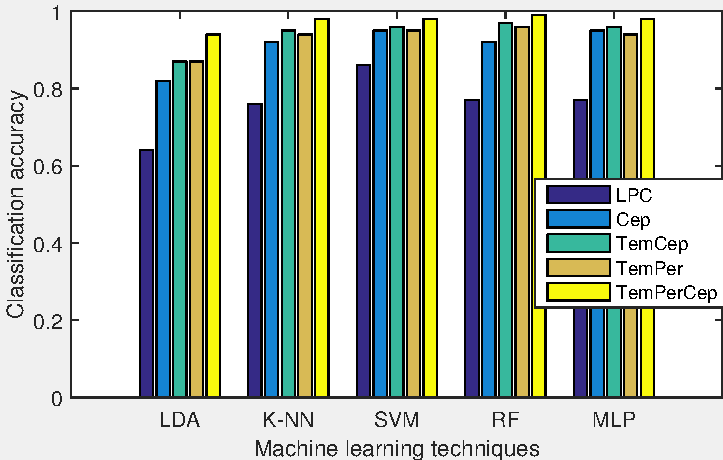
\includegraphics[width=0.6\linewidth]{image/Ch4/diffFeature.pdf}}
\caption[Classification results with different feature sets]{Classification results with different feature sets using the window size of 64 samples}
\label{diffFeature} 
\end{figure}


\subsection{Effects of different machine learning techniques}
Figure~\ref{diffClassifier} shows the frog call classification performance of 
$TemPerCep$ with different machine learning techniques. The high classification results in term of the accuracy, sensitivity and specificity measure of different classifiers indicates good classification performance. It can be observed that RF achieves the best classification performance, while the classification performance of LDA is the lowest. Meanwhile, the classification performance of SVM and MLP is very good, which might be that the features and classifiers are quite suitable. It can be seen from Figure~\ref{diffClassifier} that frog call classification with different machine learning techniques can achieve good performance with our enhanced feature set, because the classification accuracy is very high. It can also be noted that RF can be highly recommended for classification of frog calls due to the highest classification accuracy.



\begin{figure}[htb!] % Example image
\center{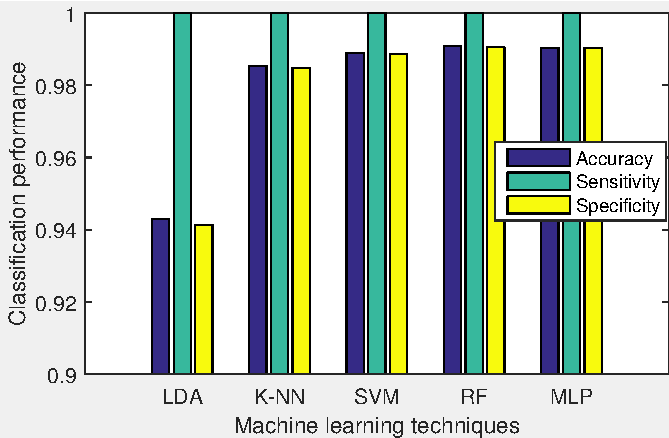
\includegraphics[width=0.6\linewidth]{image/Ch4/diffClassifier.pdf}}
\caption{Results of different classifiers}
\label{diffClassifier} 
\end{figure}



\subsection{Effects of different window size for MFCCs and perceptual features}
As we know, the window size has an effect on the MFCCs and perceptual features. Therefore, a different window size will lead to different classification performance (Figures~\ref{diffWinSize1} and \ref{diffWinSize2}). The window size used for the test is 32, 64, 128, 256, because the syllable length of some frog species is less than 512 samples.
It is found that the best classification performance for MFCCs is achieved with window size of 64 samples. For \textit{TemPer}, the window size of 64 obtains the best classification performance. 
It also can be observed that SVM and RF achieve the best classification performance. Moreover, different window sizes of MFCCs have a larger variation than \textit{TemPer} features, which might be because temporal features have a high weight in \textit{TemPer} for the classification task.

\begin{figure}[htb!] % Example image
\center{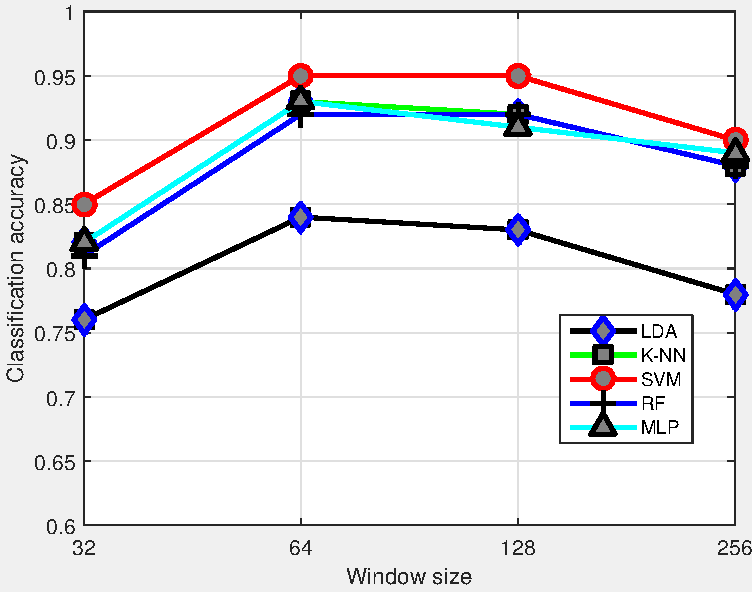
\includegraphics[width=0.6\linewidth]{image/Ch4/windowSizeMFCC.pdf}}
\caption{Classification results of MFCCs with different window sizes}
\label{diffWinSize1} 
\end{figure}

\begin{figure}[htb!] % Example image
\center{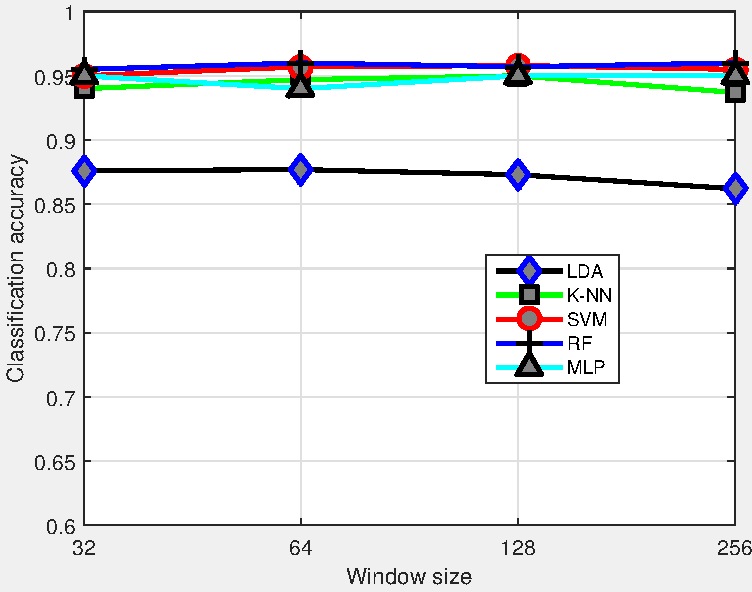
\includegraphics[width=0.6\linewidth]{image/Ch4/windowSizeTemPer.pdf}}
\caption{Classification results of TemPer with different window sizes}
\label{diffWinSize2} 
\end{figure}

\subsection{Effects of noise}
To further evaluate the robustness of our proposed feature set, white noise with different signal-to-noise (SNR) of 40 dB, 30 dB, 20 dB, 10 dB, 0dB, and -10 dB is added to the frog calls. Because this chapter focuses on the evaluation of features rather than the segmentation method, the artificial noise is added after syllable segmentation. Since SVM has shown good performance for frog call classification in 3.3.1, we only use SVM to test the effects of different levels of artificial noise. The classification results of different levels of noise contamination are shown in Figure~\ref{diffNoise}. It is found from Figure~\ref{diffNoise}, that MFCCs (Cep) are very sensitive to background noise, compared with other feature sets. Comparing \textit{TemCep} with \textit{TemPer}, it can be observed that perceptual features have a better anti-noise ability than the cepstral feature. It is also found that LPCs have a good anti-noise ability when SNR is larger than 10, but the classification accuracy quickly decreases when SNR is smaller than 10. 


\begin{figure}[htb!] % Example image
\center{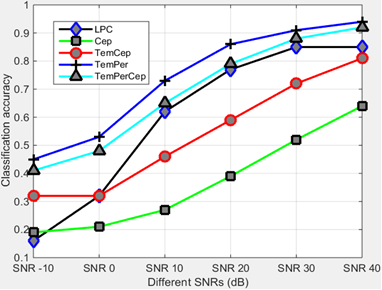
\includegraphics[width=0.6\linewidth]{image/Ch4/affectNoise.png}}
\caption{Sensitivity for different features for different levels of noise contamination}
\label{diffNoise} 
\end{figure}


\section{Discussion}
Table~\ref{my-label} shows the classification performance of previous methods. Since previous studies often used different datasets to perform the classification task, this research implemented all those features and applied them to the used dataset with the same classifier (SVM). Compared with those previous methods, this proposed enhanced feature set significantly outperforms other methods. Therefore, it can be concluded that the results of this research stand above the current classification performance. From the table, we can also observe that MFCCs are the most popular feature that has been used for frog call classification. Among all used machine learning techniques, SVM shows the superior performance and is widely used for the classification task. It can be found that the classification accuracy of \textit{TemPerCep} does not show significant improvement when compared with MFCCs. However, combining temporal and perceptual features with cepstral features greatly improves the anti-noise ability of MFCCs.

\begin{table}[h]
\centering
\caption{Comparison with previous used feature sets}
\label{my-label}
\resizebox{\textwidth}{!}{
\begin{tabular}{lll}
\hline\hline
Ref. & Feature                                                                                                                                                           & Accuracy (\%) \\ \hline
 \citep{juan2009frogs, yuan2013frog}    & LPCs                                                                                                                                                              &     93.5     \\ 
\citep{lee2006automatic, Xie1504:Acoustic, jaafar2013automatic, bedoya2014automatic}  & MFCCs                                                                                                                                                             &     94.9     \\ 
\citep{han2011acoustic}     & \begin{tabular}[c]{@{}l@{}} Spectral centroid, Shannon entropy, \\ R$\acute{e}$nyi entropy \end{tabular}  &    75.6      \\ 
\citep{Xie1504:Acoustic}    & \begin{tabular}[c]{@{}l@{}}Syllable duration, dominant frequency, \\ oscillation rate, frequency modulation, \\ energy modulation     \end{tabular}                        &    92.3    \\ 
 \citep{Huang20141}    & \begin{tabular}[c]{@{}l@{}}Spectral centroid, signal bandwidth, \\  spectral roll-off,  threshold-crossing rate, \\ spectral flatness, and average energy\end{tabular} &  95.8        \\  
 Our feature set    &                                                                                                                                        \textit{TemPerCep} &    99.1     \\ \hline\hline
\end{tabular}
}
\end{table}



\section{Summary and limitations}

In this chapter, a novel fused feature set was proposed to classify frog calls in high SNR recordings with five machine learning algorithms.
After segmenting continuous recordings into individual syllables, a variety of acoustic features are extracted from each syllable. Then, different features are combined to construct different feature sets. Finally, five machine learning techniques are used to classify frog calls in high SNR recordings with different feature sets. Classification results demonstrate that a fusion of temporal, spectral and cepstral features outperforms the state-of-the-art features used for frog call classification in high SNR recordings. Compared to temporal and spectral features, cepstral features achieve a higher classification accuracy when used individually, but are sensitive to the background noise. Therefore, we aim to develop a novel cepstral features with a good anti-noise ability in the subsequent analysis.


%In this chapter, a novel enhanced feature set was proposed to classify frog calls with various machine learning techniques. 
%Our proposed enhanced feature set shows the best classification accuracy and has good anti-noise ability. Meanwhile, the SVM and RF outperform the traditional LDA and kNN classifiers. Therefore, it is suitable to combine \textit{TemPerCep} with SVM or RF to build a frog call classification system. Ecologists can apply the proposed classification system to long-term frog recordings. Then, the long-term change of frog species richness can be reflected by the classification results. 
%
%Since the MFCCs feature shows a good classification performance, but a bad anti-noise ability, we can modify MFCCs to improve the anti-noise ability. After transforming frog audio data into its spectrogram representation, the visual inspection motivates us to use image processing techniques for studying frog calls. Also, a wider variety of frog audio data from different geographical and environmental conditions will be tested in future experiments.
